% !TeX program = pdflatex
% !TeX root = Isolate.tex

\documentclass[../FeynCalcManual.tex]{subfiles}
\begin{document}
\hypertarget{isolate}{
\section{Isolate}\label{isolate}\index{Isolate}}

\texttt{Isolate[\allowbreak{}expr]} substitutes abbreviations
\texttt{KK[\allowbreak{}i]} for all \texttt{Plus[\allowbreak{}...]}
(sub-sums) in \texttt{expr}. The inserted \texttt{KK[\allowbreak{}i]}
have head \texttt{HoldForm}.
\texttt{Isolate[\allowbreak{}expr,\ \allowbreak{}varlist]} substitutes
\texttt{KK[\allowbreak{}i]} for all subsums in \texttt{expr} which are
free of any occurrence of a member of the list \texttt{varlist}. Instead
of \texttt{KK} any other head or a list of names of the abbreviations
may be specified with the option \texttt{IsolateNames}.

\subsection{See also}

\hyperlink{toc}{Overview}, \hyperlink{isolatenames}{IsolateNames},
\hyperlink{collect2}{Collect2}.

\subsection{Examples}

\begin{Shaded}
\begin{Highlighting}[]
\NormalTok{t0 }\ExtensionTok{=}\NormalTok{ Isolate}\OperatorTok{[}\FunctionTok{a} \SpecialCharTok{+} \FunctionTok{b}\OperatorTok{]}
\end{Highlighting}
\end{Shaded}

\begin{dmath*}\breakingcomma
\text{KK}(19)
\end{dmath*}

\begin{Shaded}
\begin{Highlighting}[]
\NormalTok{t1 }\ExtensionTok{=}\NormalTok{ Isolate}\OperatorTok{[}\NormalTok{(}\FunctionTok{a} \SpecialCharTok{+} \FunctionTok{b}\NormalTok{) }\FunctionTok{f} \SpecialCharTok{+}\NormalTok{ (}\FunctionTok{c} \SpecialCharTok{+} \FunctionTok{d}\NormalTok{) }\FunctionTok{f} \SpecialCharTok{+} \FunctionTok{e}\OperatorTok{,} \FunctionTok{f}\OperatorTok{]}
\end{Highlighting}
\end{Shaded}

\begin{dmath*}\breakingcomma
e+f \;\text{KK}(19)+f \;\text{KK}(20)
\end{dmath*}

\begin{Shaded}
\begin{Highlighting}[]
\FunctionTok{StandardForm}\OperatorTok{[}\NormalTok{t1}\OperatorTok{]}
\end{Highlighting}
\end{Shaded}

\begin{dmath*}\breakingcomma
e+f \;\text{KK}[19]+f \;\text{KK}[20]
\end{dmath*}

\begin{Shaded}
\begin{Highlighting}[]
\OperatorTok{\{}\NormalTok{t0}\OperatorTok{,}\NormalTok{ t1}\OperatorTok{,} \FunctionTok{ReleaseHold}\OperatorTok{[}\NormalTok{t1}\OperatorTok{]\}}
\end{Highlighting}
\end{Shaded}

\begin{dmath*}\breakingcomma
\{\text{KK}(19),e+f \;\text{KK}(19)+f \;\text{KK}(20),f (a+b)+f (c+d)+e\}
\end{dmath*}

\begin{Shaded}
\begin{Highlighting}[]
\NormalTok{Isolate}\OperatorTok{[}\FunctionTok{a}\OperatorTok{[}\FunctionTok{z}\OperatorTok{]}\NormalTok{ (}\FunctionTok{b} \SpecialCharTok{+} \FunctionTok{c}\NormalTok{ (}\FunctionTok{y} \SpecialCharTok{+} \FunctionTok{z}\NormalTok{)) }\SpecialCharTok{+} \FunctionTok{d}\OperatorTok{[}\FunctionTok{z}\OperatorTok{]}\NormalTok{ (}\FunctionTok{y} \SpecialCharTok{+} \FunctionTok{z}\NormalTok{)}\OperatorTok{,} \OperatorTok{\{}\FunctionTok{a}\OperatorTok{,} \FunctionTok{d}\OperatorTok{\},}\NormalTok{ IsolateNames }\OtherTok{{-}\textgreater{}}\NormalTok{ fF}\OperatorTok{]}
\end{Highlighting}
\end{Shaded}

\begin{dmath*}\breakingcomma
\text{fF}(22) a(z)+\text{fF}(21) d(z)
\end{dmath*}

\begin{Shaded}
\begin{Highlighting}[]
\FunctionTok{Information}\OperatorTok{[}\NormalTok{fF}\OperatorTok{]}
\end{Highlighting}
\end{Shaded}

\FloatBarrier
\begin{figure}[!ht]
\centering
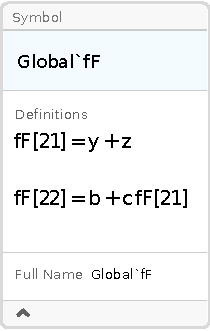
\includegraphics[width=0.6\linewidth]{img/0gi2hdxwlvyo6.pdf}
\end{figure}
\FloatBarrier

\begin{Shaded}
\begin{Highlighting}[]
\NormalTok{Global\textasciigrave{}fF}
\end{Highlighting}
\end{Shaded}

\begin{dmath*}\breakingcomma
\text{fF}
\end{dmath*}

\begin{Shaded}
\begin{Highlighting}[]
\NormalTok{fF}\OperatorTok{[}\DecValTok{26}\OperatorTok{]} \ExtensionTok{=} \FunctionTok{y} \SpecialCharTok{+} \FunctionTok{z}
\end{Highlighting}
\end{Shaded}

\begin{dmath*}\breakingcomma
y+z
\end{dmath*}

\begin{Shaded}
\begin{Highlighting}[]
\NormalTok{fF}\OperatorTok{[}\DecValTok{27}\OperatorTok{]} \ExtensionTok{=} \FunctionTok{b} \SpecialCharTok{+} \FunctionTok{c} \FunctionTok{HoldForm}\OperatorTok{[}\NormalTok{fF}\OperatorTok{[}\DecValTok{26}\OperatorTok{]]}
\end{Highlighting}
\end{Shaded}

\begin{dmath*}\breakingcomma
b+c \;\text{fF}(26)
\end{dmath*}

\begin{Shaded}
\begin{Highlighting}[]
\NormalTok{Isolate}\OperatorTok{[}\FunctionTok{a} \SpecialCharTok{{-}} \FunctionTok{b} \SpecialCharTok{{-}} \FunctionTok{c} \SpecialCharTok{{-}} \FunctionTok{d} \SpecialCharTok{{-}} \FunctionTok{e}\OperatorTok{,}\NormalTok{ IsolateNames }\OtherTok{{-}\textgreater{}} \FunctionTok{l}\OperatorTok{,}\NormalTok{ IsolateSplit }\OtherTok{{-}\textgreater{}} \DecValTok{15}\OperatorTok{]}
\end{Highlighting}
\end{Shaded}

\begin{dmath*}\breakingcomma
l(24)
\end{dmath*}

\begin{Shaded}
\begin{Highlighting}[]
\FunctionTok{Clear}\OperatorTok{[}\NormalTok{t0}\OperatorTok{,}\NormalTok{ t1}\OperatorTok{,} \FunctionTok{l}\OperatorTok{,}\NormalTok{ fF}\OperatorTok{]}
\end{Highlighting}
\end{Shaded}

\end{document}
